\chapter{O Projeto CDME e o Projeto Ótimo}
\label{cap:CDME}

% ->¨Veio de um incentivo do governo de apoio financeiro à produção de conteúdos digitais educacionais, em um contexto de aumento de aumento de investimento na inclusão digital de alunos de escolas públicas
% -> Softwares para esse propósito costumam ser pagos e oferecidos principalmente em inglês e esquema de mensalidade, o que é dramático em situações de inflação e desvalorização da moeda.
% -> software livre e com curva de aprendizado suave: professor e aluno não precisam se preocupar com implementação de tecnologia alguma.
% -> contém mais de 60 atividades que contemplam as mais diversas áreas da matemática.

% -> cdme estava pra ser incluído no portal do professor, segundo \citeonline{bortolossiaulas}

% Um capítulo sobre o projeto CDME (histórico, contexto, objetivos e o que ele alcançou) 

A década de 2010 foi marcada por um avanço em políticas educacionais que investiam na inclusão digital dos alunos e professores de escola públicas. O estado do Rio de Janeiro forneceu, por exemplo, um notebook com acesso a internet via conexão 3G a cada professor da rede estadual. Com esse movimento de inclusão também se investiu em produção de conteúdos educacionais digitais multimídia. Uma iniciativa, por exemplo, foi um edital no valor de 75 milhões de reais do Ministério de Educação e do Ministério da Ciência, em meados de 2007 que focava no segmento do ensino médio, e contemplava as áreas de química, biologia, e português~\cite{cdmebortolossi2016conteudos}.

Esse edital buscava a produção de conteúdos de qualidade, fácil acesso e boas orientações metodológicas e gratuito, que pudesse servir de alternativa aos recursos pagos, normalmente em sistema de assinatura, que se tornam inviáveis até mesmo para escolas e universidade.


\section{O Projeto CDME}

% MINISTÉRIO DA CIÊNCIA E TECNOLOGIA
% MINISTÉRIO DA EDUCAÇÃO
% EDITAL DE SELEÇÃO Nº 1/2007
% CHAMADA PÚBLICA PARA APOIO FINANCEIRO À PRODUÇÃO DE CONTEÚDOS EDUCACIONAIS DIGITAIS MULTIMÍDIA

Dentre os projetos contemplados no edital de Chamada Pública Para Apoio Financeiro À Produção De Conteúdos Educacionais Digitais Multimídia (Edital 1/2007), conjunto do Ministério de Ciência e Tecnologia e Ministério da Educação~\cite{editalCDME}, estava o projeto CDME\footnote{Conteúdos Digitais para o Ensino e Aprendizagem da Matemática do Ensino Médio} da Universidade Federal Fluminense, contemplado com financiamento de 220 mil reais para o desenvolvimento de mais de 60 atividades multimídia, experimentos e clipes de áudio educacionais para a área de Matemática, de utilização livre e gratuita por professores. O projeto propunha atividades fechadas que o professor poderia usar com os seus alunos, indo diretamente para o foco do problema sem ter que se preocupar com a montagem ou implementação da atividade, e chegou a ser cogitado para ser incluído na no Portal do Professor do MEC~\cite{bortolossiaulas}. \\

O Projeto Ótimo foi disponibilizado no endereço \url{http://www.cdme.im-uff.mat.br/pot/pot-html/pot-br.html}. Como explicaremos no capítulo~\ref{cap:partetecnica}, este projeto foi implementado utilizando a tecnologia dos applets java, que atualmente perdeu o suporte nos navegadores modernos. Como já dissemos, o foco deste trabalho foi a atualização das atividades do projeto, e a nova versão pode ser encontrada no link \url{https://fellipessanha.github.io/CDME-javascript/pot/}.\\

As atividades propostas no CDME abrangem diversos conteúdos de Matemática e Estatística abordados no Ensino Médio. Entre os temas estão: 

\begin{itemize}
    \item Geometria Espacial, em atividades como "Uma Pletora de Poliedros", que permitia manipular e visualizar diversos tipos de poliedros, e "Jogo da Tomografia", cujo objetivo era identificar um objeto visualizando apenas duas projeções ortogonais em um eixo;
    
    \item Estatística, nas atividades "Distribuição de Frequências e Seus Gráficos", que descreve como gráficos são feitos a partir de dados estatísticos, e "Pesquisas Estatísticas no Dia a Dia", que detalha alguns dados estatísticos importantes do Brasil;
    
    \item Funções, como em "Variação da Função Exponencial", que contém uma série de exercícios que abordam a natureza da função exponencial,
    
    \item Otimização, no grupo de atividades intitulado "Projeto Ótimo", que consiste em diversas situações de otimização, com atividades associadas; entre outros.
\end{itemize}

Neste trabalho, nos concentraremos no grupo de atividades intitulado ``Projeto Ótimo", com uma pequena apresentação sobre as atividades, seus objetivos e métodos, uma discussão sobre a temática de otimização no Ensino Médio e o problema da atualização destas atividades para as novas tecnologias de recursos computacionais. 

\section{O Projeto Ótimo}


\begin{figure}[htb!]
    \centering
    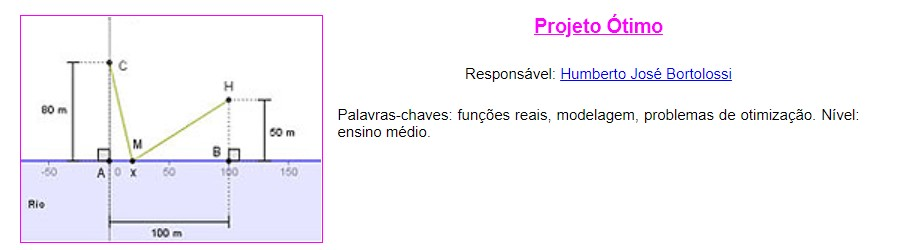
\includegraphics[width=\textwidth]{media/CDME-projeto-otimo.jpg}
    \caption{Thumbnail do Projeto Ótimo no site do CDME}
    \label{fig:projotimo}
\end{figure}

O Projeto Ótimo~(Figura \ref{fig:projotimo}) consiste de 21 módulos de problemas de otimização de uma variável acompanhados de construções GeoGebra, contextualizando a situação-problema, além de gráficos que relacionam as variáveis do domínio do problema com a imagem no contra-domínio. Os problemas exploram conceitos como domínio, imagem, gráfico de função, entre outros, estimulando conexões entre os aspectos algébrico, numérico, geométrico e verbal da função real. Para que o foco permaneça no processo de otimização propriamente dito, todas estas atividades possuem solução única e facilmente identificável como tal dentro do domínio.

Esses módulos vêm acompanhados de um documento com exercícios sugeridos que, caso o professor escolha usar, podem ser modificados para se adequarem aos alunos. Além disso, o professor pode utilizar as atividades de diversas maneiras: junto aos alunos em sala de aula; utilizando um projetor ou monitor; como atividade de casa após uma introdução em aula; em laboratório de informática da escola, deixando que os alunos discutam entre si e com o professor.
\\

A otimização --- tema do Projeto -- é, de maneira geral, o processo de maximizar ou minimizar o valor de uma função, através da uma escolha viável de suas variáveis segundo as condições impostas pela situação em que o problema se insere. Tais problemas são relevantes por serem extremamente comuns em praticamente qualquer área de atuação profissional: um empresário busca maximizar lucros; um engenheiro busca maior eficiência na produção; empresas de logística buscam maximizar a eficiência do roteamento de seus veículos. 
\\

Além de contextos humanos e profissionais, problemas de otimização também aparecem em contextos naturais: uma bolha de sabão é tal que a sua superfície é a mínima para um dado volume; a luz sempre percorre a distância que minimize a distância percorrida; e um objeto sempre tende ao equilíbrio em um ponto que minimize a sua energia potencial.

A grande relevância e recorrência deste tipo de problemas torna indispensável sua abordagem em sala de aula. Muitos dos alunos terão que \textit{otimizar} alguma tarefa ao longo de suas vidas, e a experiência de reconhecer domínios e contra-domínios, elaborar e modelar uma lei de função, aprender técnicas que facilitem suas resoluções, quando vista em sala de aula, pode acrescentar muito na formação escolar. 
\\

Cada módulo do Projeto Ótimo consiste de duas ou mais atividades. Uma atividade trata da otimização da situação apresentada, por exemplo, determinar a medida da base que maximiza a área de um triângulo, dado um perímetro fixo. Outra, aborda a modelagem geral de um problema, por exemplo, determinar a lei de formação de um triângulo de perímetro fixo, em função de sua base, seguindo o exemplo anterior. Essas atividade são acompanhados por uma simulação computacional gráfica da situação, que permite que o aluno interaja com o problema e tenha um melhor entendimento de suas particularidades e limitações. As situações também são acompanhadas de formulários de acompanhamento do aluno, que propõem reflexões adicionais sobre a estrutura do problema de otimização naquele contexto.

\begin{figure}[htb]
    \begin{subfigure}[b]{0.47\textwidth}
    \centering
    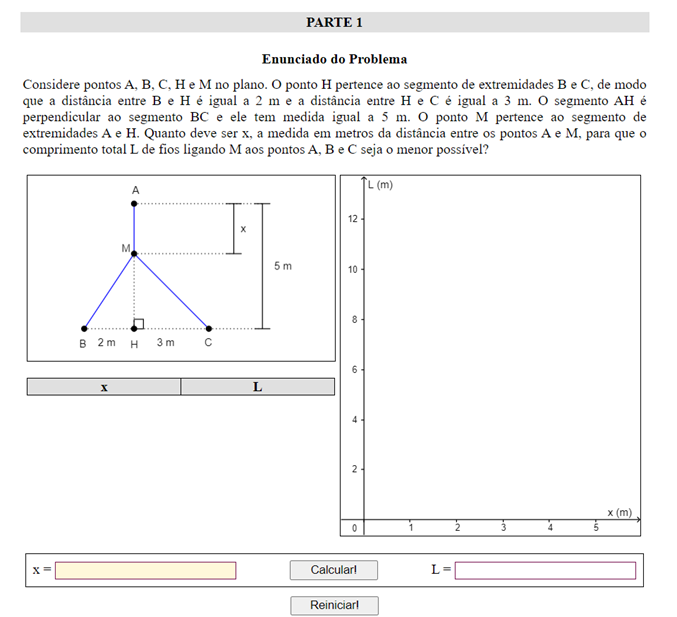
\includegraphics[width=\textwidth]{media/CDME-prob-geometrico-12.png}
    \caption{Exemplo de atividade do Projeto Ótimo sem nenhuma entrada/}
    \label{fig:otimo13-11}
    \end{subfigure}
    % 
    \hfill
    % 
    \begin{subfigure}[b]{0.47\textwidth}
    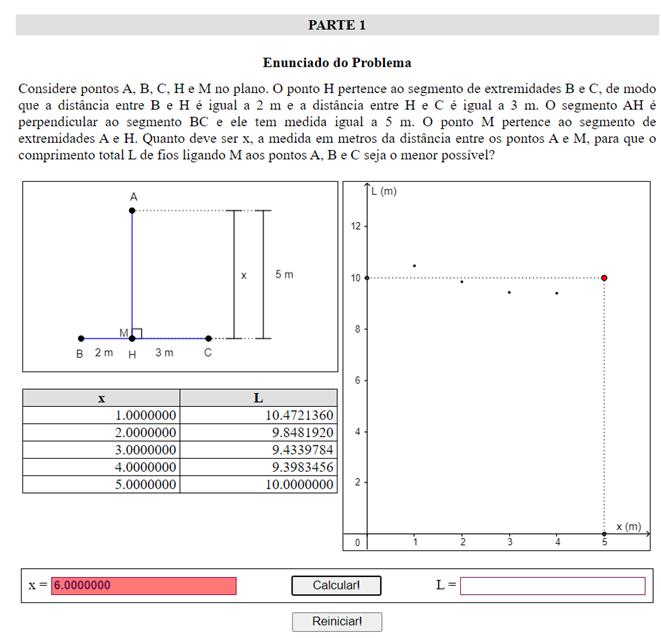
\includegraphics[width=\textwidth]{media/CDME-prob-geometrico-11.png}
    \caption{Exemplo de atividade do Projeto Ótimo após entradas válidas.}
    \label{fig:otimo13-12}
    \end{subfigure}
    \caption{Primeira parte do módulo 6: ``Um Problema Geométrico".}
    \label{fig:otimo13-1}
    
\end{figure}

\begin{figure}
\begin{subfigure}[b]{0.47\textwidth}
    \centering
    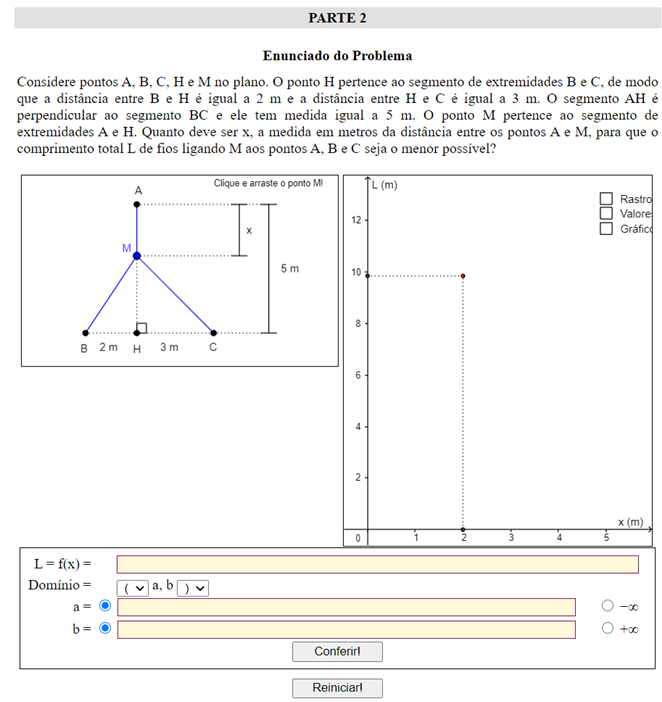
\includegraphics[width=8cm]{media/CDME-prob-geometrico-21.png}
    \caption{Atividade sem rastro nem linha do gráfico aparente}
\end{subfigure}
% 
\hfill
% 
\begin{subfigure}[b]{0.47\textwidth}
    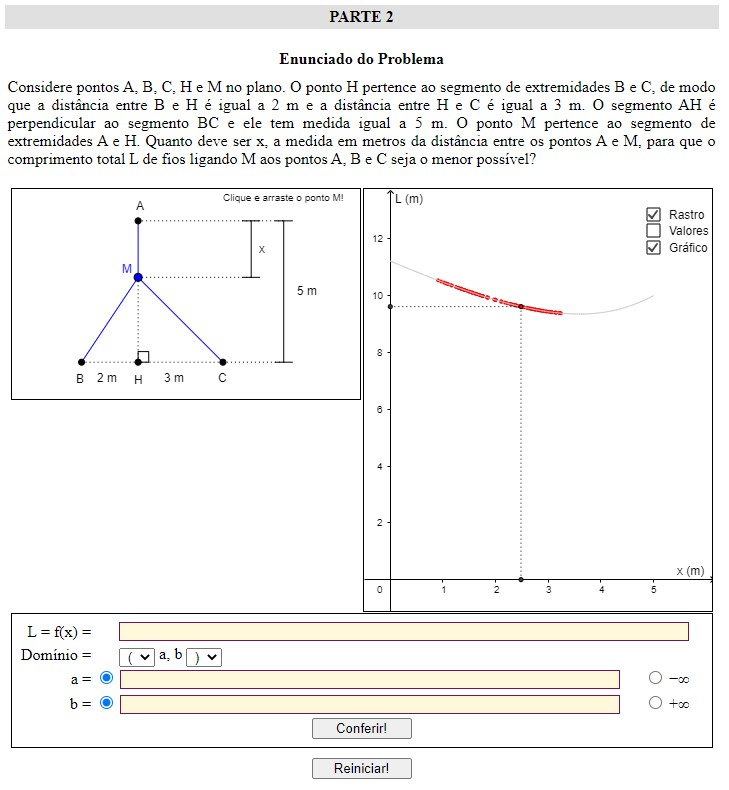
\includegraphics[width=8cm]{media/CDME-problema-geometric-grafico-rastro.jpg}
    \caption{Atividade com a linha do gráfico e alguns pontos do rastro aparentes aparente}
\end{subfigure}
    \caption{Segunda parte do módulo 6: ``Um Problema Geométrico"}
    \label{fig:otimo13-2}
\end{figure}

Um exemplo da estrutura citada no parágrafo anterior se encontra nas Figuras~\ref{fig:otimo13-1} e~\ref{fig:otimo13-2}. Na primeira parte o aluno deve buscar o valor da variável que otimiza o problema proposto. O valor da variável pode ser calculado ou estimado com o apoio das construções do GeoGebra, que exibem a situação-problema adaptada para o valor estimado da variável e a representação dessa estimativa no gráfico em uma tabela, como mostrado nas Figuras~\ref{fig:otimo13-11} e \ref{fig:otimo13-12}. Na segunda parte o aluno deve descrever a lei de formação da função e seu domínio, utilizando os conhecimentos que obteve na primeira etapa e uma nova construção GeoGebra, que permite interação clicando e arrastando nos pontos que representam a variável do domínio, ao mesmo tempo em que o gráfico é atualizado com o rastro deixado pelas variações. Também é possível ver diretamente o gráfico da função (Figura~\ref{fig:otimo13-2}).


Essa abordagem incentiva que o aluno entenda o problema e aprenda Matemática por meio de sua resolução. O entendimento de uma situação-problema traz benefícios como o de relacionar o pensar matemático com uma gama maior de contextos, estimular a capacidade do aluno de reconhecer ideias ou conceitos matemáticos, e ajuda a construir as relações entre as diversas ideias matemáticas que permeiam um dado problema~\cite{schroeder1989developing}.

Outra questão que vem à tona no Projeto Ótimo é a da representação matemática em contextos eletrônicos. A maior parte dos alunos está acostumada a representar os conceitos matemáticos através de símbolos --- $\sqrt{16}=4$, $2\pi\theta$, ou $2^3=8$, por exemplo --- que não são possíveis de escrever com teclados convencionais. Por isso, o aluno deve se familiarizar com a noção de que a representação de uma determinada operação ou conceito pode variar dependendo do contexto, e também se familiarizar com a maneira de escrevê-las da maneira que a programação do site entenda. Por exemplo, em contextos computacionais, é usual uma notação baseada no conceito de função, como em \texttt{sqrt()} para representa raiz quadrada. As operações aritméticas também possuem outras notações, como \^{} para representar potência, \texttt{*} para produto, etc. Também se faz necessário maior uso de parênteses para explicitar a precedência de operações, por exemplo \texttt{(x\^{}(25)+1)/(3\^{}2)} em vez de $\frac{x^{25}+1}{3^2}$.

\section{As atividades do Projeto Ótimo}

A seguir apresentaremos os 21 módulos do Projeto Ótimo, com seus respectivos enunciados e acompanhados de um pequeno comentário destacando pontos interessantes em cada um.

\begin{itemize}
    \item Módulo 1: ``O Problema da Cerca"
    
    ``Com 80 metros de cerca um fazendeiro deseja circundar uma região retangular junto a um rio para confinar alguns animais. O lado da região retangular junto a margem do rio não é cercado. Quanto deve ser x, a medida em metros da base da região retangular, para que a área cercada A seja a maior possível?”.
    
    É uma contextualização clássica de problema de otimização, que trabalha simultaneamente as noções de perímetro e área, evidenciando suas relações e diferenças com elementos muito comuns: cerca e área de terreno. Tem como pré-requisitos área e perímetro de retângulo, o Teorema de Pitágoras.
    
    
    \item Módulo 2: ``O Problema do Barbante: Quadrado e Círculo"
    
    ``Um fio de barbante de 10 metros de comprimento pode ser usado ou para construir um quadrado, ou para construir um círculo ou ele pode ser cortado em dois pedaços (não necessariamente de mesmo tamanho) de modo que um dos pedaços é usado para construir um quadrado e o outro pedaço é usado para construir um círculo. Quanto deve ser x, a medida em metros do pedaço do barbante usado para construir o quadrado, para que a soma S das áreas das figuras produzidas seja a maior possível? Quanto deve ser x, a medida em metros do pedaço do barbante usado para construir o quadrado, para que a soma S das áreas das figuras produzidas seja a menor possível?”.

    Trata da comparação entre a relação área-perímetro entre figuras geométricas diferentes --- círculo e quadrado, no caso. Tem como pré-requisitos área e perímetro de quadrados, área e perímetro de círculos, o Teorema de Pitágoras. 
    
    \item Módulo 3: ``O Problema do Barbante: Quadrado e Triângulo"
    
    % \begin{citacao}
    ``Um fio de barbante de 10 metros de comprimento pode ser usado ou para construir um quadrado, ou para construir um triângulo equilátero ou ele pode ser cortado em dois pedaços (não necessariamente de mesmo tamanho) de modo que um dos pedaços é usado para construir um quadrado e o outro pedaço é usado para construir um triângulo equilátero. Quanto deve ser x, a medida em metros do pedaço do barbante usado para construir o quadrado, para que a soma S das áreas das figuras produzidas seja a maior possível? Quanto deve ser x, a medida em metros do pedaço do barbante usado para construir o quadrado, para que a soma S das áreas das figuras produzidas seja a menor possível?”
    % \cite{cdme-pot}
    % \end{citacao}
    
    Módulo análogo ao anterior, agora com as figuras quadrado e triângulo equilátero. Serve como complemento e reforço para que o aluno entenda de onde vêm as proporções que maximizam a soma da área das figuras. Trata da comparação entre a relação área-perímetro entre figuras geométricas diferentes --- círculo e quadrado, no caso. Tem como pré-requisitos área e perímetro de quadrados, área e perímetro de triângulos equiláteros, o Teorema de Pitágoras. 
    
    \item Módulo 4: ``O Problema da Janela Normanda"
    
    ``Uma janela normanda tem o formato da justaposição de um semicírculo sobre um retângulo. Considerando as janelas normandas com perímetro igual a 9 m, quanto deve ser x, a medida em metros da base do retângulo que compõe a janela, para que a área A da janela seja a maior possível?”
    
    Aborda a relação que se apresenta entre o perímetro e a área de uma figura geométrica. Tem como pré-requisitos perímetro e área de retângulos, perímetro e área de semicírculos.
    
    \item Módulo 5: ``O Problema do Triângulo Isósceles"
    
    ``Considerando os triângulos isósceles com dois lados de medidas iguais a 3 m, quanto deve ser x, a medida em metros da base triângulo isósceles, para que a área A do triângulo seja a maior possível?”.
    
    Esse módulo traz a relação implícita entre ângulo e base de um triângulo com dois lados fixos, podendo ser usada para instigar o pensamento trigonométrico. tem como pré-requisitos área e perímetro de triângulos, o Teorema de Pitágoras.
    
    \item Módulo 6: ``Um Problema Geométrico"
    
     ``Considere pontos A, B, C, H e M no plano. O ponto H pertence ao segmento de extremidades B e C, de modo que a distância entre B e H é igual a 2 m e a distância entre H e C é igual a 3 m. O segmento AH é perpendicular ao segmento BC e ele tem medida igual a 5 m. O ponto M pertence ao segmento de extremidades A e H. Quanto deve ser x, a medida em metros da distância entre os pontos A e M, para que o comprimento total L de fios ligando M aos pontos A, B e C seja o menor possível?”
     
     É o primeiro módulo a não citar área, focando no teorema de Pitágoras e na relação cartesiana da distância entre um ponto fixo e um outro que varia em um eixo. Tem como pré-requisitos distância entre pontos no plano, o Teorema de Pitágoras.
    
    \item Módulo 7: ``O Problema do Caminho para A Horta"
    
    ``Um agricultor está em sua casa C situada a 80 metros da margem retilínea de um rio. Ele quer encher primeiro o seu regador de água em um ponto M na margem deste rio e, depois, se dirigir para sua horta H, situada a 50 metros da margem do rio. A distância entre os pés A e B das perpendiculares traçadas de C e H sobre a margem do rio é igual a 100 metros. Considere um sistema de coordenadas onde A = (0, 0), B = (100, 0), C = (0, 80), H = (100, 50) e M = (x, 0). Quanto deve ser x, a abscissa do ponto M sobre o eixo x, para que o comprimento d do trajeto casa (C), rio (M) e horta (H) seja o menor possível?”
    
    Pela primeira vez, o enunciando traz explicitamente a notação utilizada em planos cartesianos, e apresenta os primeiros conceitos relacionados à Geometria Analítica, instigando esse tipo de pensamento na cabeça do aluno sem necessariamente se aprofundar. O exercício do módulo em si é semelhante ao anterior, então valem os mesmos comentários, e os pré-requisitos são distância entre pontos no plano, o Teorema de Pitágoras.
    
    \item Módulo 8: ``O Problema da Distância entre Ponto e Reta"
    
    ``Dado um ponto A no plano cartesiano, quanto deve ser x para que a distância d entre A e M = (x, -2x + 4) (um ponto da reta y = -2x + 4) seja a menor possível?”
    
    O módulo traz, inserindo o conceito de função dentro do exercício de função, uma situação inteiramente composta de objetos Matemáticos. Dá, assim, oportunidade para o aluno desenvolver a sua capacidade de abstração, com o auxílio do gráfico. Tem como pré-requisito distância entre pontos no plano.
    
    \item Módulo 9: ``O Problema da Distância entre Ponto e Parábola"

    ``Dado um ponto A no plano cartesiano, quanto deve ser x para que a distância d entre A e M = (x, x$^2$) (um ponto da parábola y = x$^2$) seja a menor possível?”
    
    Assim como no módulo anterior, este propõe uma atividade contextualizada apenas com abstrações Matemáticas. Ao trabalhar com um objeto pouco frequente em problemas que envolvem distâncias, traz um questionamento mais aprofundado sobre a definição de distância de um ponto a um conjunto, no caso a parábola. Busca-se na atividade o ponto da parábola cuja distância ao ponto dado é mínima, isto é, o ponto que realiza a distância entre parábola e ponto.
    
    % caracterizar a distância de um ponto a um objeto, uma determinada curva a menor distância, ponto que pode ser resolvido intuitivamente e sem mais reflexões no módulo anterior. Tem como pré-requisito distância entre pontos no plano.
    
    \item Módulo 10: ``O Problema do Retângulo: Área e Perímetro"
    
    ``Considerando os retângulos de área igual a 3 m$^2$, quanto deve ser x, a medida em metros da base do retângulo, para que o perímetro y do retângulo seja o menor possível?”
    
    Aqui o projeto aborda novamente a relação de área e perímetro, dessa vez invertendo a relação proposta anteriormente, avaliando o perímetro em função da área. Tem como pré-requisitos área e perímetro de retângulo.
    
    \item Módulo 11: ``O Problema do Retângulo Inscrito num Círculo"
    
    ``Queremos encaixar (inscrever) dentro de um círculo um retângulo com a maior área possível. Se o círculo tem 3 metros de raio, quanto deve ser x, a medida em metros da base do retângulo, para que a área A do retângulo seja a maior possível?”
    
    Voltando a tratar o conceito de área em Geometria Plana, o módulo trabalha a ideia do problema de otimização com restrição com esse problema simples, oferecendo uma representação gráfica do problema. Tem como pré-requisitos área e perímetro de retângulos, o Teorema de Pitágoras.

    \item Módulo 12: ``O Problema do Triângulo Inscrito num Círculo"
    
    ``Queremos encaixar (inscrever) dentro de um círculo um triângulo isósceles com a maior área possível. Se o círculo tem 3 metros de raio, quanto deve ser x, a medida em metros da altura do triângulo, para que a área A do triângulo seja a maior possível?”
    
    Similarmente ao módulo anterior, explora a variação da área de um triângulo isósceles, com a restrição de estar inscrito em um círculo de raio fixo. Traz um exercício muito interessante envolvendo o teorema de Pitágoras, e tem com pré-requisitos área de triângulos, e o já mencionado Teorema de Pitágoras.
    
    \item Módulo 13: ``O Problema da Bobina do Transformador"
    
    ``Na construção de um transformador de corrente alternada, insere-se na bobina circular do transformador um núcleo de ferro cuja seção transversal tem o formato de uma cruz. É importante que esta seção transversal tenha a maior área possível. Se o raio da seção transversal circular da bobina mede 18 milímetros e se x representa a metade da medida, em milímetros, dos lados da cruz cujas extremidades estão sobre a seção circular, quanto deve ser x para que a área A da cruz seja a maior possível?"

    Esse módulo apresenta uma contextualização muito interessante vinda da engenharia, e começa a trabalhar com áreas não triviais. Nela o aluno deve quebrar a área da \textit{cruz} em áreas menores que ele consegue calcular, estimulando o pensamento de \textit{dividir para conquistar}, tão importante na matemática. Tem como pré-requisitos área de retângulos, o Teorema de Pitágoras.
    
    \item Módulo 14: ``O Problema da Caixa"
    
    ``Quadrados iguais são cortados dos cantos de uma folha de papelão retangular medindo 30 cm por 50 cm. As abas que sobram são então dobradas para cima de modo a formar uma caixa sem tampa. Quanto deve ser x, a medida em centímetros dos lados dos quadrados que são retirados da folha de papelão, para que o volume V da caixa seja o maior possível?”
    
    A partir desse módulo as atividades passam a tratar de geometria em três dimensões. O projeto inicia essa sequência com uma atividade que trata da relação entre área e volume em uma figura geométrica espacial. Tem como pré-requisitos área e perímetro de retângulos, volume de prismas retos quadrangulares.
    
    \item Módulo 15: ``O Problema da Caixa com Tampa"
    
    ``Um fabricante quer construir caixas com tampa a partir de uma folha de papelão retangular medindo 10 cm por 16 cm. Para construir a caixa, dois quadrados e dois retângulos são removidos dos cantos da folha de papelão. As abas que sobram são então dobradas para cima de modo a formar uma caixa com tampa. Quanto deve ser x, a medida em centímetros dos lados dos quadrados que são retirados da folha de papelão, para que o volume V da caixa seja o maior possível?”
    
    O módulo é muito similar ao anterior, com a diferença do formato da figura tratada. O fato de a caixa não ter tampa altera o corte feito, e assim muda a quantidade máxima de papelão que pode ser utilizada em uma situação dessa, excelente para promover o pensamento crítico. Tem como pré-requisitos área e perímetro de retângulos, volume de prismas retos quadrangulares.
    
    \item Módulo 16: ``O Problema do Bebedouro"
    
    ``Um bebedouro será construído na forma de um prisma reto cuja altura mede 7 m e cujas bases são trapézios. Cada trapézio tem base menor e laterais de medidas sempre iguais a 1 m. Se x representa a medida, em radianos, do ângulo entre uma lateral e uma altura de cada um dos dois trapézios congruentes usados na construção do bebedouro, quanto deve ser x para que a forma do bebedouro correspondente tenha o maior volume V possível?”
    
    Esse módulo se mostra interessante para abordar trigonometria, já que precisamos de uma maneira de relacionar os comprimentos das arestas com a variável sobre a qual temos algum controle: o ângulo. A questão do bebedouro se enchendo de água também traz a possibilidade de abordar o tema da semelhança entre sólidos. Tem como pré-requisitos área de triângulos, área de retângulos, trigonometria no triângulo retângulo, volume de prismas retos, o Teorema de Pitágoras.
    
    \item Módulo 17: ``O Problema da Embalagem Piramidal"
    
    ``Um fabricante quer construir uma embalagem no formato de uma pirâmide regular de base quadrada a partir de uma folha de papelão quadrada medindo 2 m por 2 m. Para construir a embalagem, triângulos isósceles são removidos das laterais da folha de papelão. As pontas que sobram são então dobradas para cima de modo a formar uma pirâmide regular de base quadrada. Quanto deve ser x, a metade da medida em metros da diagonal da base quadrada da pirâmide, para que o volume V da embalagem seja o maior possível?”
    
    Outro módulo que se estende sobre a relação entre área e volume de um sólido específico através da planificação, oferecendo uma estratégia interessante para a obtenção da planificação de uma pirâmide a partir de uma superfície quadrada. Tem como pré-requisitos elementos métricos do triângulo isósceles, elementos métricos do quadrado, volume de pirâmides regulares, o Teorema de Pitágoras.
    
    \item Módulo 18: ``O Problema do Cone"
    
    ``Um copo no formato cônico é feito com um disco circular de papel, de centro O, do qual foi retirado um setor circular AOM e os lados OA e OM foram unidos. Os lados OA e OM têm medida 7 cm. Quanto deve ser x, a medida em radianos do ângulo AOM, para que o volume V do copo seja o maior possível?”
    
    O último módulo explicitamente sobre relação entre área e volume, agora introduzindo um sólido não poliédrico, explora a relação da área lateral do cone como o seu volume. Tem como pré-requisitos perímetro de arcos de círculo, volume de cones circulares, o Teorema de Pitágoras.
    
    \item Módulo 19: ``O Problema do Cilindro Inscrito numa Esfera"
    
    ``Queremos encaixar (inscrever) dentro de uma esfera um cilindro circular reto com o maior volume possível. Se a esfera tem 3 metros de raio, quanto deve ser x, a medida em metros do raio da base do cilindro, para que o volume V do cilindro seja o maior possível?”
    
    Módulo análogo ao número 11, possibilita a discussão das simetrias de figuras geradas a partir de rotações de uma figura plana. Os pré-requisitos são volume de cilindros circulares, o Teorema de Pitágoras.
    
    \item Módulo 20: ``O Problema do Cone Inscrito numa Esfera"
    
    ``Queremos encaixar (inscrever) dentro de uma esfera um cone circular reto com o maior volume possível. Se a esfera tem 3 metros de raio, quanto deve ser x, a medida em metros da altura do cone, para que o volume V do cone seja o maior possível?”
    
    Um exercício parecido com o do Módulo 11, agora trabalhado em 3 dimensões. Possibilita essa discussão da Geometria Plana presente em seções de figuras tridimensionais. Tem como pré-requisitos volume de cones circulares, o Teorema de Pitágoras.
    
    \item Módulo 21: ``O Problema da Pirâmide Inscrita numa Esfera"
    
    ``Queremos encaixar (inscrever) dentro de uma esfera uma pirâmide regular de base quadrada com o maior volume possível. Se a esfera tem 3 metros de raio, quanto deve ser x, a medida em metros da altura da pirâmide, para que o volume V da pirâmide seja o maior possível?”
    
    O último módulo atualmente mistura a noção de poliedro --- a pirâmide inscrita --- com sólidos não poliédricos --- a esfera ---, que pode promover questionamentos interessantes se comparado com a atividade anterior. Quando pontos da pirâmide encostam na esfera, e como essa informação difere do caso do cone e o cilindro inscritos? Tem como pré-requisitos volume de pirâmides regulares, o Teorema de Pitágoras.
\end{itemize}

\begin{figure}
    \centering
    
    \begin{subfigure}{0.3\textwidth}
    \centering
    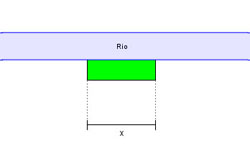
\includegraphics[width=.9\textwidth]{icones-modulos/pot-m-pce.jpg}
    \label{fig:pce-ic}
    \end{subfigure}
    \hfill
    \begin{subfigure}{0.3\textwidth}
    \centering
    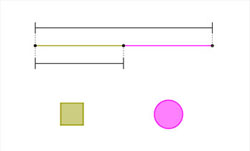
\includegraphics[width=.9\textwidth]{icones-modulos/pot-m-pbc.jpg}
    \label{fig:pbc-ic}
    \end{subfigure}
    \hfill
    \begin{subfigure}{0.3\textwidth}
    \centering
    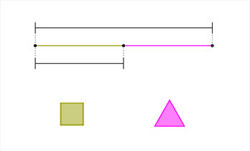
\includegraphics[width=.9\textwidth]{icones-modulos/pot-m-pbt.jpg}
    \label{fig:pbt-ic}
    \end{subfigure}
    
    \begin{subfigure}{0.3\textwidth}
    \centering
    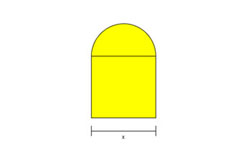
\includegraphics[width=.9\textwidth]{icones-modulos/pot-m-pjn.jpg}
    % \label{fig:pdc-ic}
    \end{subfigure}
    \hfill
    \begin{subfigure}{0.3\textwidth}
    \centering
    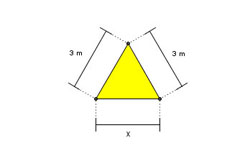
\includegraphics[width=.9\textwidth]{icones-modulos/pot-m-ptr.jpg}
    % \label{fig:pdc-ic}
    \end{subfigure}
    \hfill
    \begin{subfigure}{0.3\textwidth}
    \centering
    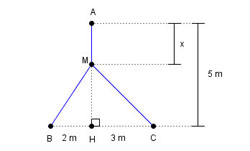
\includegraphics[width=.9\textwidth]{icones-modulos/pot-m-pge.jpg}
    \label{fig:pge-ic}
    \end{subfigure}
    
    \begin{subfigure}{0.3\textwidth}
    \centering
    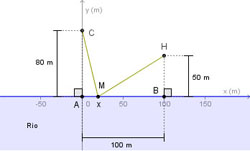
\includegraphics[width=.9\textwidth]{icones-modulos/pot-m-pch.jpg}
    % \label{fig:pch-ic}
    \end{subfigure}
    \hfill
    \begin{subfigure}{0.3\textwidth}
    \centering
    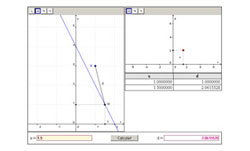
\includegraphics[width=.9\textwidth]{icones-modulos/pot-m-pre.jpg}
    \label{fig:pre-ic}
    \end{subfigure}
    \hfill
    \begin{subfigure}{0.3\textwidth}
    \centering
    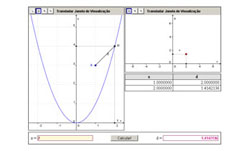
\includegraphics[width=.9\textwidth]{icones-modulos/pot-m-ppa.jpg}
    \label{fig:ppa-ic}
    \end{subfigure}
    
    \begin{subfigure}{0.3\textwidth}
    \centering
    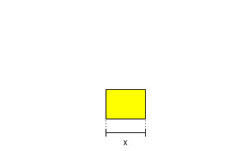
\includegraphics[width=.9\textwidth]{icones-modulos/pot-m-rap.jpg}
    \label{fig:rap-ic}
    \end{subfigure}
    \hfill
    \begin{subfigure}{0.3\textwidth}
    \centering
    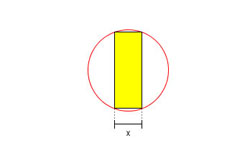
\includegraphics[width=.9\textwidth]{icones-modulos/pot-m-crt.jpg}
    \label{fig:crt-ic}
    \end{subfigure}
    \hfill
    \begin{subfigure}{0.3\textwidth}
    \centering
    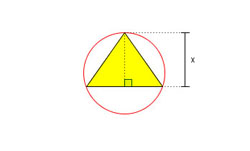
\includegraphics[width=.9\textwidth]{icones-modulos/pot-m-ctr.jpg}
    \label{fig:ctr-ic}
    \end{subfigure}
    
    \begin{subfigure}{0.3\textwidth}
    \centering
    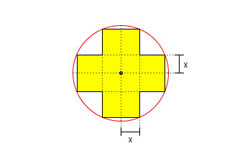
\includegraphics[width=.9\textwidth]{icones-modulos/pot-m-pbo.jpg}
    \label{fig:pbo-ic}
    \end{subfigure}
    \hfill
    \begin{subfigure}{0.3\textwidth}
    \centering
    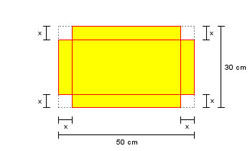
\includegraphics[width=.9\textwidth]{icones-modulos/pot-m-pdc.jpg}
    \label{fig:pdc-ic}
    \end{subfigure}
    \hfill
    \begin{subfigure}{0.3\textwidth}
    \centering
    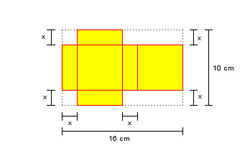
\includegraphics[width=.9\textwidth]{icones-modulos/pot-m-pct.jpg}
    \label{fig:pct-ic}
    \end{subfigure}
    
    
    \begin{subfigure}{0.3\textwidth}
    \centering
    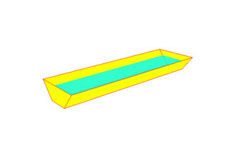
\includegraphics[width=.9\textwidth]{icones-modulos/pot-m-pbe.jpg}
    \label{fig:pbe-ic}
    \end{subfigure}
    \hfill
    \begin{subfigure}{0.3\textwidth}
    \centering
    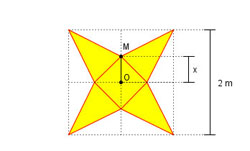
\includegraphics[width=.9\textwidth]{icones-modulos/pot-m-pep.jpg}
    \label{fig:pep-ic}
    \end{subfigure}
    \hfill
    \begin{subfigure}{0.3\textwidth}
    \centering
    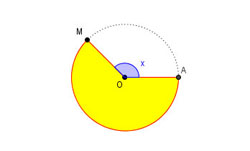
\includegraphics[width=.9\textwidth]{icones-modulos/pot-m-pco.jpg}
    \label{fig:pco-ic}
    \end{subfigure}
    
    \begin{subfigure}{0.3\textwidth}
    \centering
    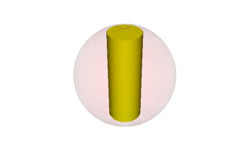
\includegraphics[width=.9\textwidth]{icones-modulos/pot-m-eci.jpg}
    \label{fig:eci-ic}
    \end{subfigure}
    \hfill
    \begin{subfigure}{0.3\textwidth}
    \centering
    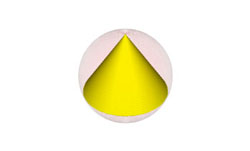
\includegraphics[width=.9\textwidth]{icones-modulos/pot-m-eco.jpg}
    \label{fig:eco-ic}
    \end{subfigure}
    \hfill
    \begin{subfigure}{0.3\textwidth}
    \centering
    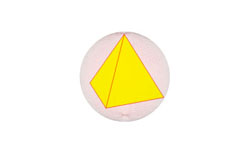
\includegraphics[width=.9\textwidth]{icones-modulos/pot-m-epi.jpg}
    \label{fig:epi-ic}
    \end{subfigure}
    
    \caption{Thumbnails dos módulos do Projeto Ótimo}
    \label{fig:icones-pot}
    
    
\end{figure}